% !TeX document-id = {c68f4be8-c497-43e0-82df-e9ebfbea9577}
% !TeX TXS-program:pdflatex = pdflatex -synctex=1 -interaction=nonstopmode --shell-escape %.tex
% новая команда \RNumb для вывода римских цифр
\documentclass[a4paper,12pt]{article}
\usepackage{amssymb}
\usepackage{amsmath}
\usepackage{amsthm} 
\usepackage{caption}
\usepackage{misccorr}
\usepackage[noadjust]{cite}
\usepackage{cmap} 
\usepackage[utf8]{inputenc}
\usepackage[T2A]{fontenc}
\usepackage[english, russian]{babel}
\usepackage{graphics}
\usepackage{graphicx}
\usepackage{textcomp}
\usepackage{verbatim}
\usepackage{makeidx}
\usepackage{geometry}
\usepackage{float}
\usepackage{bm}
\usepackage{esint}
\usepackage{mathtools}
\usepackage{graphicx}
\usepackage{listings}
\usepackage{courier}
\usepackage{multirow}
\usepackage{graphicx}

\lstset{basicstyle=\fontsize{10}{10}\selectfont,breaklines=true}

\newcommand{\specchapter}[1]{\chapter*{#1}\addcontentsline{toc}{chapter}{#1}}
\newcommand{\specsection}[1]{\section*{#1}\addcontentsline{toc}{section}{#1}}
\newcommand{\specsubsection}[1]{\subsection*{#1}\addcontentsline{toc}{subsection}{#1}}
\newcommand{\RNumb}[1]{\uppercase\expandafter{\romannumeral #1\relax}}
\newcommand{\jj}{\righthyphenmin=20 \justifying}


% геометрия
\geometry{pdftex, left = 2cm, right = 2cm, top = 2.5cm, bottom = 2.5cm}

\setcounter{tocdepth}{4} % фикс переноса 
\righthyphenmin = 2
\tolerance = 2048

\begin{document}
\thispagestyle{empty}

\noindent \begin{minipage}{0.15\textwidth}
	
\includegraphics[width=\linewidth]{b_logo}
\end{minipage}
\noindent\begin{minipage}{0.9\textwidth}\centering
	\textbf{Министерство науки и высшего образования Российской Федерации}\\
	\textbf{Федеральное государственное бюджетное образовательное учреждение высшего образования}\\
	\textbf{«Московский государственный технический университет имени Н.Э.~Баумана}\\
	\textbf{(национальный исследовательский университет)»}\\
	\textbf{(МГТУ им. Н.Э.~Баумана)}
\end{minipage}

\noindent\rule{18cm}{3pt}
\newline\newline
\noindent ФАКУЛЬТЕТ $\underline{\text{«Информатика и системы управления»}}$ \newline\newline
\noindent КАФЕДРА $\underline{\text{«Компьютерные системы и сети»}}$\newline\newline
\noindent НАПРАВЛЕНИЕ ПОДГОТОВКИ $\underline{\text{«09.03.04 Программная инженерия»}}$\newline\newline\newline\newline\newline


\begin{center}
	\noindent\begin{minipage}{1.3\textwidth}\centering
	\Large\textbf{  ОТЧЕТ }\newline
	\textbf{по лабораторной работе №3}\newline\newline
	\end{minipage}
\end{center}

\noindent\textbf{Название:} $\underline{\text{Исследование регистров}}$\newline\newline
\noindent\textbf{Дисциплина:} $\underline{\text{Архитектура ЭВМ}}$\newline\newline\newline\newline\newline

\begin{center}
	\begin{tabular}{ccccc}
		Студент: & $\underline{\text{ИУ7-43Б}}$ & $\underline{\text{~~~~~~~~~~~}}$ & $\underline{\text{26.04.2020}}$ & $\underline{\text{А. В. Романов}}$ \\
		 & \footnotesize группа & \footnotesize подпись & \footnotesize дата  & \footnotesize (И. О. Фамилия) \\
		  &  &  &  & \\
		Преподаватель: & \textbf{} & $\underline{\text{~~~~~~~~~~~}}$ & $\underline{\text{~~~~~~~~~~~~}}$ & $\underline{\text{А. Ю. Попов}}$ \\
		&  & \footnotesize подпись & \footnotesize дата  & \footnotesize (И. О. Фамилия) \\
	\end{tabular}
\end{center}


\begin{center}
	\vfill
	Москва~---~\the\year
~г.
\end{center}
\clearpage

\section{Цель работы} Изучение принципов построения регистров сдвига, способов преобразования параллельного кода в последовательный и обратно, сборка схем регистров сдвига их экспериментальное исследование. 

\section{Исследование регистра сдвига}
Схема пятиразрядного регистра сдвига вправо.
\begin{center}
	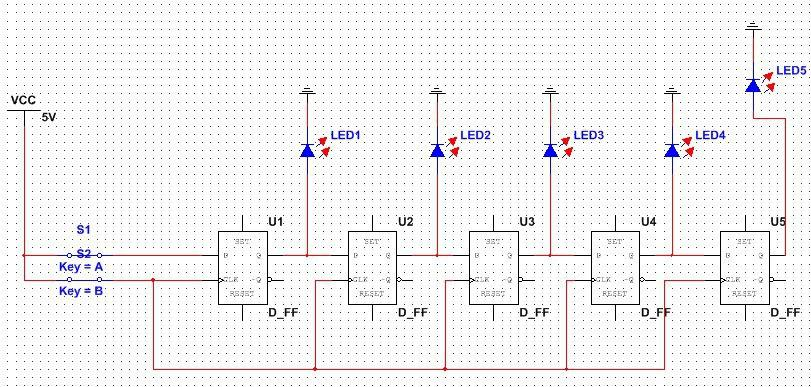
\includegraphics[scale=0.6]{../screens/1.jpg}
\end{center}

\noindent Файл: 1.ms\newline\newline

\noindent Схема пятиразрядного регистра сдвига вправо в циклическом режиме
\begin{center}
	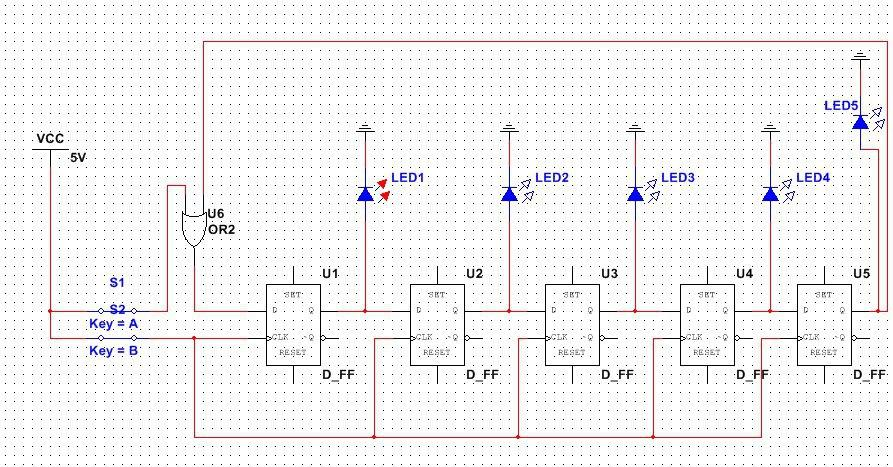
\includegraphics[scale=0.55]{../screens/2.jpg}
\end{center}

\noindent Файл: 2.ms\newline\newline

\clearpage
\noindent Схема пятиразрядного регистра сдвига влево
\begin{center}
	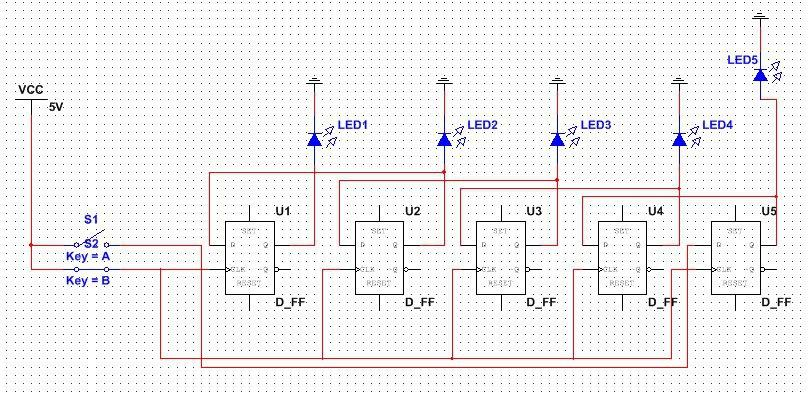
\includegraphics[scale=0.65]{../screens/3.jpg}
\end{center}

\noindent Файл: 3.ms\newline\newline

\noindent Схема пятиразрядного регистра сдвига влево в циклическом режиме
\begin{center}
	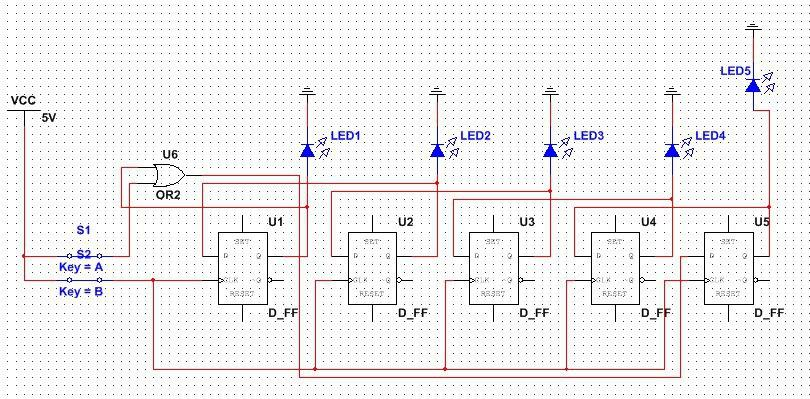
\includegraphics[scale=0.65]{../screens/4.jpg}
\end{center}

\noindent Файл: 4.ms\newline

\noindent Количество триггеров и выходных сигналов равно разряду регистра. Чтобы получить циклический режим, соединяются первый и последний триггер. 

\section{Исследование универсального регистра на ИС К555ИР11 (74LS194)}

\begin{center}
	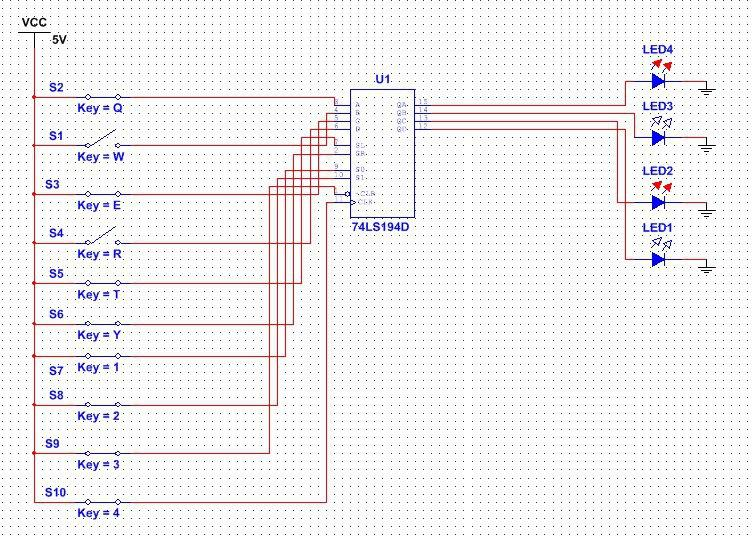
\includegraphics[scale=0.6]{../screens/5.jpg}
	
	""\newline
	
	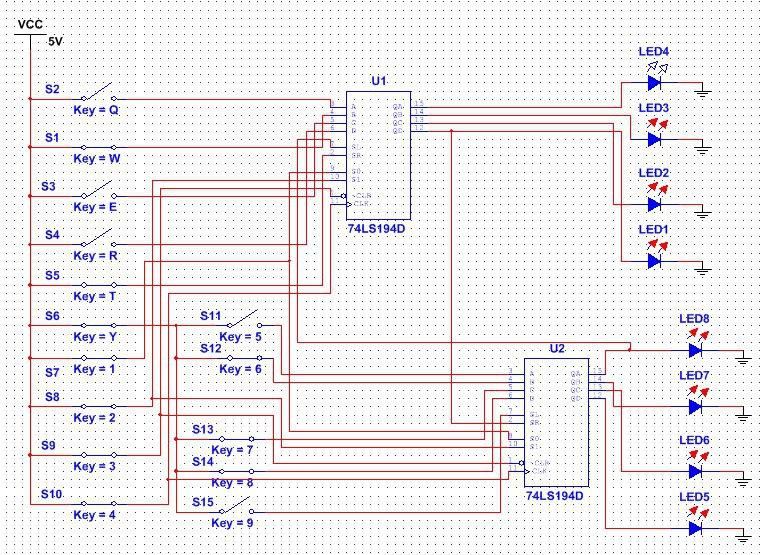
\includegraphics[scale=0.6]{../screens/6.jpg}
\end{center}

\noindent Файлы: 5.ms и 6.ms\newline

\noindent С помощью таких регистров можно обрабатывать информацию, подаваемую на входы. См. контрольный вопрос №6.

\section{Вывод}

\noindent При выполнении этой лабораторной работы я изучил работу регистров сдвига (вправо и влево, а так же циклических), универсального регистра.

\section{Контрольные вопросы}

\noindent\textbf{1.} Что называется регистром? Какие функции выполняют регистры?\newline

\noindent\textbf{Регистр} - операционный узел ЭВМ, предназначенный для выполнения микроопераций записи, хранения, преобразования и считывания слова (или части слова) данных и простейших поразрядных логических операций. Регистры осуществляют кратковременное хранение информации в течение одного или нескольких циклов работы устройства\newline

\noindent\textbf{2.} Как классифицируются регистры по способу ввода-вывода информации? \newline

\noindent По способу ввода и вывода:

- параллельные (или регистры памяти), 

- последовательные, 

- параллельно-последовательные, 

- последовательно-параллельные, 

- универсальные или многофункциональные\newline

\noindent\textbf{3.} Как работает параллельный регистр с однофазным и парафазным приемом информации?\newline

\noindent \textbf{В однофазных} -- каждый разряд передается по одной линии (в виде прямого значения $D_{i}$ или инверсии)\newline

\noindent \textbf{В парафазных} -- каждый разряд передается по двум линями (прямым $D_{i}$ и инверсными значениям в каждом из рарзядов.)\newline

%\clearpage
\noindent\textbf{4.} Какие типы триггеров применяются в регистрах сдвига?\newline

\noindent Регистры сдвига с однофазной синхронизацией строятся на cинхронных D-триггерах с динамическим управлением записью.
\newline

\noindent\textbf{5.} Как работает регистр сдвига, выполненный на триггерах с двухступенчатым запоминанием информации? Как работает регистр сдвига на триггерах с динамическим управлением записью?\newline

\noindent Входные данные $D_{R}$ в последовательном коде поступают на вход D триггера нулевого разряда регистра сдвига. Для передачи сигналов из одного разряда в другой (при сдвиге вправо), выход $Q$ тригера разряда $i$, соединен с входом $D$, который имет разряд $i + 1$. С каждым тактовым сигналом $C$, поступающим на входы $C$ всех триггеров регистра, происходит сдвиг разрядов, то есть перезапись.
\newline

\noindent\textbf{6.} Объясните работу универсального регистра сдвига.\newline

\noindent По входам $S0$ и $S1$ можно выполнять некоторые операции. Таблицу операций привожу ниже.

\begin{center}
	\begin{tabular}{ | l | l | l | p{1cm} |}
		\hline
		$S1$ & $S0$ & Режим работы  \\ \hline
		
		0 & 0 & Хранение  \\ \hline
		0 & 1 & Сдвиг вправо  \\ \hline
		1 & 0 & Сдвиг влево  \\ \hline
		1 & 1 & Ввод данных (пареллельный)  \\ 
		\hline
	\end{tabular}
\end{center}


\noindent Входы $D_{0}$ - $D_{7}$ -- ячейки памяти в регистре. $D_{R}$ ($SR$) и $D_{L}$ ($SL$) -- входы ввода данных в регистр последовательным кодом при сдвигах вправо и влево. Операясь на эти операции, можно реализовать некоторые арифметические операции. А с помощью арифметических операций можно построить что-нибудь более сложное.


\end{document}